\documentclass[12pt,a4paper]{article}
\usepackage[utf8]{inputenc}
\usepackage[T1]{fontenc}
\usepackage[brazilian]{babel}
\usepackage{amsmath}
\usepackage{amsfonts}
\usepackage{amssymb}
\usepackage{graphicx}
\usepackage{outlines}
\usepackage{indentfirst}
\usepackage{datetime}
\setlength{\parskip}{.5em}
\usepackage{enumitem}
\setlist{nosep}
\usepackage[section]{placeins}
\def\tam{0.6}
\usepackage{draftwatermark}
\SetWatermarkText{DRAFT}
\SetWatermarkScale{1}
\usepackage[all]{nowidow}
\nowidow
\noclub
\usepackage[scale=1.5]{ccicons}
\usepackage{authblk}
\usepackage{hyperref}



\title{Dicas para Provas de Aula}
\author{Geraldo Xexéo}
\affil{\url{xexeo@ufrj.br} \\
    \url{http://xexeo.net}}
\date{\ccbyncsa\  - \today}


\author{Geraldo Xexéo}
\title{Dicas de Como Fazer Slides Acadêmicos}

\begin{document}



\maketitle

\begin{abstract}
    Este artigo fornece dicas de como fazer slides de aula, para apresentações em congressos e para defesas de projeto final, dissertações, teses e exames de qualificação.
\end{abstract}

\tableofcontents


\section{Introdução}

Este documento é um guia com dicas para o uso de slides em apresentações no Programa de Engenharia de Sistemas e Computação.

Ele é construído como um guia básico, do mínimo necessário, e razoavelmente conservador.

Este material está disponível no GitHub, junto com material de apoio, como slides Power Point que eu uso e distribuo: \url{https://github.com/xexeo/DicasSlidesAcademicos}.

Outra questão importante neste documento: ele é criado por um usuário do \textit{Power Point} que tem experiência com o \texttt{beamer}, o estilo de apresentações do \LaTeX. Muitos softwares de apresentação são altamente compatíveis com o \textit{Power Point}, seguindo a mesma filosofia de trabalho, baseado no WYSIWYG. Outros softwares, como o Prezi\footnote{\url{https://prezi.com/}} podem exigir outra forma de pensar, porém muitas dicas dadas aqui continuam válidas. A Seção \ref{sec:ferramentas} discute um pouco os principais softwares e características importantes do seu uso.

Usarei o termo geral \textit{apresentação} para uma aula, defesa de tese ou apresentação de artigo em congresso.

Os slides são mostrados com frames para delimitar o seu tamanho.



\section{O estilo dos slides}

Os slides devem apresentar uma identidade conjunta. Para isso devem ser usados estilos apropriados, que estão disponíveis nas ferramentas de criação, ou se criar um estilo novo. A Figura \ref{fig:tres} mostra três slides diferentes em tipo e que mantêm uma identidade conjunta por meio de cores, fontes e rodapés.

É muito importante usar o recurso de estilos do software escolhido, porque ele permite mudar rapidamente a imagem geral da apresentação sem ter que alterar slide a slide. No repositório GitHub disponibilizo  arquivos \textit{Power Point} que na verdade são o mesmo conteúdo\footnote{\url{https://github.com/xexeo/DicasSlidesAcademicos/tree/main/Slides}}, aplicando estilos diferentes.

Esse estilo deve possuir vários tipos de slides. A aula deve usar mais de um desses tipos, tanto para cumprir papéis posicionais, como o título e título de seção, quanto para não ficar monótona. Os tipos principais são:
\begin{itemize}
    \item título;
    \item o título de seção;
    \item o slide de uma coluna, o mais comum;
    \item o slide de duas colunas;
    \item o slide de duas colunas com títulos, e
    \item o slide só com título, usado para figuras e composições.
\end{itemize}




\begin{figure}[htb]
    \centering
    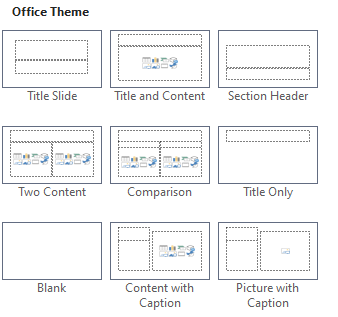
\includegraphics[width=0.5\linewidth]{imagens/tiposbasicosdopp}
    \caption{Slides básicos disponíveis no Power Point}
    \label{fig:tiposbasicosdopp}
\end{figure}

A Figura \ref{fig:tiposbasicosdopp}, copiada do \textit{Power Point} mostra esses seis tipos principais e mais alguns disponíveis para uma apresentação em branco, como o slide branco, e dois modelos com legenda. Já a Figura \ref{fig:vermelhao} mostra vários formatos de slides que eu criei no estilo que chamo de ``vermelhão'', mostrando uma gama de formatos que já usei.

\begin{figure}[hbt]
    \centering
    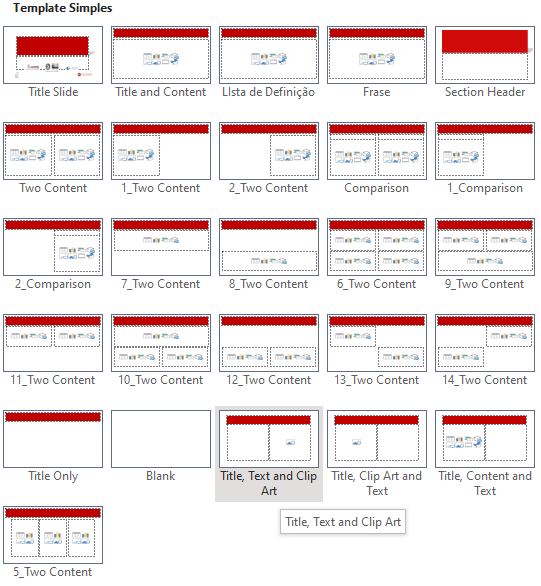
\includegraphics[width=0.5\linewidth]{imagens/vermelhao}
    \caption{Variantes de formatos de slide criados para um estilo, no Power Point.}
    \label{fig:vermelhao}
\end{figure}


Cada tipo de uso, como apresentação, aula, defesas ou exames, tem um estilo de slide mais adequado, de acordo com a necessidade de chamar atenção, e o grau de formalidade.

Em qualquer tipo de uso, porém, existem alguns objetos que devem aparecer nos slides, como a numeração e a identificação do autor e da instituição.

Os slides \textbf{devem ser numerados} e conter em cada slide o número total de slides, possivelmente no formato ``slide/total'', como em ``4/40''. Os números não podem ser pequenos, e eu favoreço números grandes, para que fique bem claro e possam, mesmo a distância, serem usados como referência. Esse número fica normalmente no rodapé (\textit{footer}) do slide. No \texttt{beamer} isso pode ser feito com o comando:

\verb|\setbeamertemplate{page number in head/foot}[totalpagenumber]|


Também é importante ter a identificação do autor. Normalmente ela inclui um e-mail ou um site.

Além disso, é interessante que, para a maioria dos usos, o estilo do slide esteja diretamente associado a uma instituição. Isso pode ser feito por meio da colocação do logo da instituição em uma posição clara.

No Power Point existem, por \textit{default}, três espaços no rodapé do slide (\textit{footer}). Um é reservado para o número. Os outros dois são possivelmente livres, sendo que um  sempre devemos usar identificar o autor. O terceiro espaço pode ser usado para o título da apresentação, o título do curso, o título do evento ou outra informação similar que se quer ressaltar.

A Figura \ref{fig:coppe} mostra um slide com todos esses elementos: o logo do PESC, o nome e e-mail do autor, o nome do curso, o número do slide em uma fonte grande e o número total de slides em uma fonte menor.



Devemos usar fontes ``limpas'', não rebuscadas, e \textbf{sem-serifa}\footnote{Serifas são as pontinhas que existem em algumas fontes. Elas estão bem visíveis no S da palavra ``slides'' desta seção.}, como Arial ou Calibri, e \textbf{corpos grandes}, 32 pts, por exemplo. Os slides das Figuras \ref{fig:coppe} e \ref{fig:teximag} seguem essa regra. Já o slide da figura \ref{fig:formulas} usa um tamanho menor para o corpo das fórmulas. Lembre que a banca, ao invés dos alunos, é mais velha e pode ter dificuldades de visão.





\subsection{Usando os logos corretos}

É \textbf{importantíssimo usar os logos corretos das instituições}. Para isso procure os logos originais e os manuais de marca.

No caso da UFRJ, houve um logo especial em 2020, para os 100 anos, e em 2021 o logo tradicional foi substituído por um logo moderno em azul. A variante vertical de uso preferencial é mostrada na Figura \ref{fig:logoufrj}. O PESC também tem um novo logo desde 2021, que é mostrado na Figura \ref{fig:logopesc}. Esse logo chegou a ser divulgado sem a referência a COPPE, e usar essa versão é errado.

\begin{figure}[hbt]
    \centering
    \subfloat[Logo vertical]{
    
\includegraphics[height=3cm]{imagens/UFRJ}\label{fig:logoufrjv}}
    \subfloat[Logo horizontal]{
    
\includegraphics[height=3cm]{imagens/UFRJH}\label{fig:logoufrjh}}
    \caption{Alguns dos logos novos da  UFRJ e partir de 2021. Existem versões com o nome completo que são de uso em contextos quando a UFRJ é menos conhecida.}
    \label{fig:logoufrj}
\end{figure}

\begin{figure}[hbt]
    \centering
    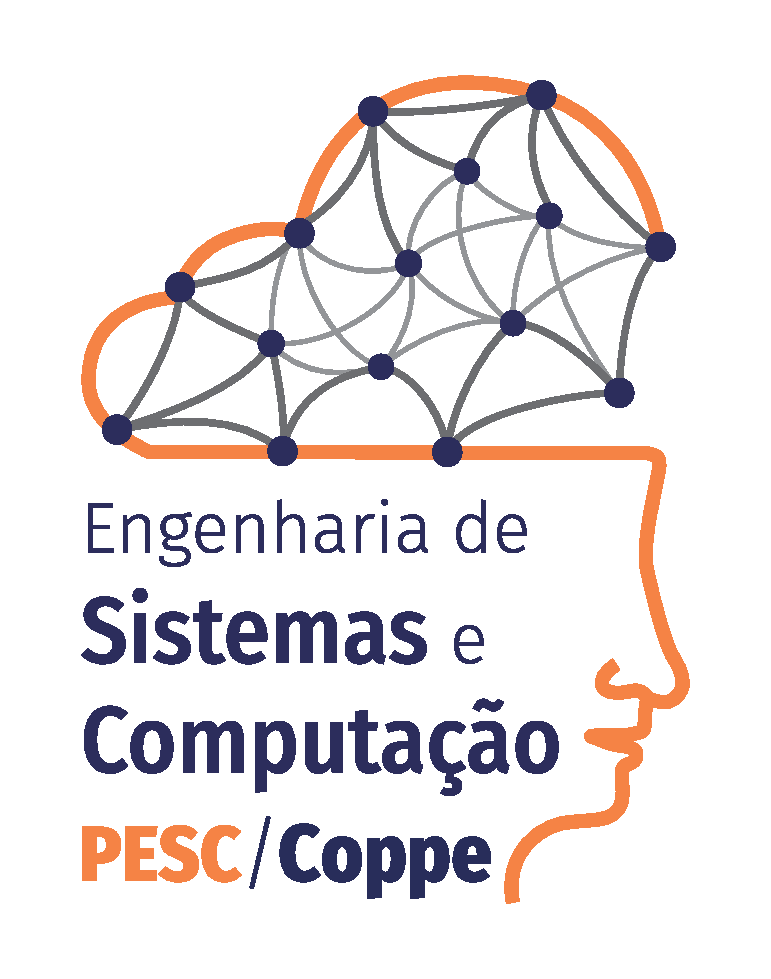
\includegraphics[height=3cm]{imagens/logoPrincipal.eps}
    \caption{Logo novo do PESC.}
    \label{fig:logopesc}
\end{figure}



No GitHub que divulga este texto é possível baixar uma apresentação simples do PESC, feita em \textit{Power Point}, que usa os logos corretos\footnote{\url{https://github.com/xexeo/DicasSlidesAcademicos/tree/main/Slides}}.



A lista de logos que eu uso é:
\begin{itemize}
    \item UFRJ: \url{https://ufrj.br/comunicacao/manuais-e-modelos/marca-da-ufrj/}
    \item COPPE: \url{https://www.coppe.ufrj.br/pt-br/a-coppe/uso-da-marca}
    \item PESC:  \url{https://www.cos.ufrj.br/index.php/pt-BR/logo-pesc}
    \item IM: não fornece o logotipo na página, porém é possível copiar. A história da marca principal está em \url{https://sites.google.com/matematica.ufrj.br/mapcabral/outros/hist%C3%B3ria-do-logotipo-do-im}
    \item DCC: não fornece o logotipo na página, mas, de qualquer maneira, será transformado no IC, com novo logotipo
    \item POLI: \url{http://www.poli.ufrj.br/marcadapolitecnica.php}
    \item LUDES: \url{https://github.com/LUDES-PESC/Generico/tree/master/Logo%20Novo%20Vers%C3%B5es}
    \item LINE: \url{https://github.com/LINE-PESC/Generico/tree/master/Logomarca%20LINE}
\end{itemize}

No GitHub deste documento estão disponíveis algumas sugestões de slides.


\subsection{Nomeando os slides}

Todo slide deve ter um \textbf{título único}. Esse espaço já vem reservado nos estilos de \textit{Power Point}.

Algumas pessoas, erroneamente, usam um título de seção que se repete nessa posição e colocam o que seria o título do slide como uma caixa-de-texto, ou como primeiro item da lista de itens do slide. Essa prática faz com que a audiência se perca em relação a onde o apresentador está. O nome e o número do slides servem não só para identificá-los, mas também como posicionamento na sequência.

É possível criar um slide com o nome da seção, mas ele deve ser menor que o nome do slide. Usando o \texttt{beamer}, o formato de slides do \LaTeX, é possível colocar no topo do slide uma mini-agenda, onde o nome da seção tem uma ênfase. As Figuras \ref{fig:sistemas} e \ref{fig:meio} mostram  slides que têm todas as seções identificadas em seu cabeçalho, sendo que a seção atual está com ênfase.

Se for necessário ter dois slides com o mesmo nome, porque um é continuação do outro, numere os slides como foi feito na Figura \ref{fig:dados}, indicando também o total de slides dessa sequência com o mesmo nome, no formato ``(n/N)''.



\subsection{Slide de contato}

Como adicional, toda apresentação deve possuir um slide final que indica um contato. Hoje, todas as minhas aulas terminam com o slide da Figura \ref{fig:fim}. Isso pode ser usado sempre para falar algo como ``quem quiser me contatar para tirar dúvidas...''.

\begin{figure}[h]
    \centering
    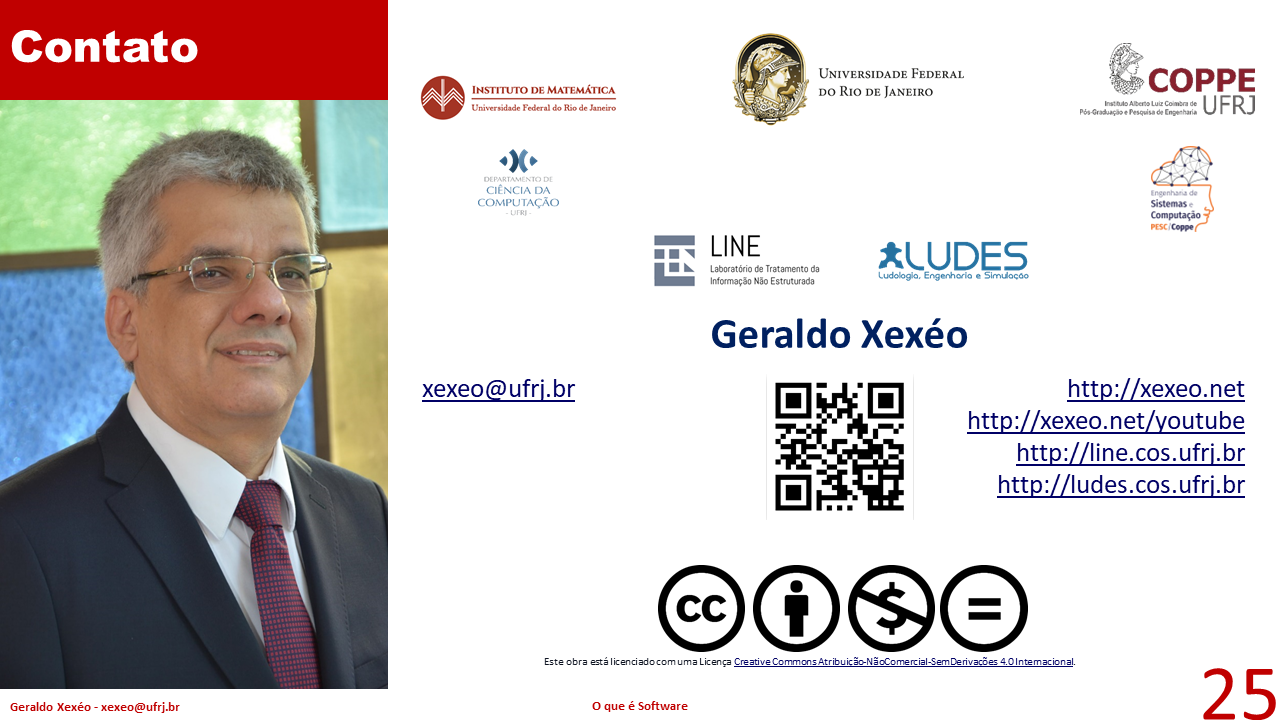
\includegraphics[width=\tam\linewidth,frame]{imagens/fim.png}
    \caption{Um slide de contato.}
    \label{fig:fim}
\end{figure}




\section{Slides de Aulas}

Nesta seção tratamos exclusivamente de slides destinados a apresentação de aulas completas sobre um assunto específico. Esse tipo de sequência é comum para professores.

\subsection{Que slides ter}

Os seguintes slides são recomendados para uma boa aula:
\begin{outline}
    \1 \textbf{Título da aula}, como na Figura \ref{fig:titulo};
    \1 \textbf{Objetivo da aula};
    \1 \textbf{Revisão} do que é necessário para entender a aula;
    \2 \textbf{Contextualizando} a aula curso
    \1 \textbf{Habilidades} específicas que serão aprendidas;
    \1 \textbf{Agenda} (ou Sumário);
    \2 A agenda ou sumário divide a aula em seções;
    \1 Um slide de \textbf{título para cada seção};
    \2 Pode ser o slide da agenda colocando ênfase na seção atual, como na Figura \ref{fig:meio};
    \1 Slides de conteúdo;
    \2 Não esqueça de uma motivação quando necessário;
    \2 Não esqueça do contexto histórico do que está sendo ensinado;
    \2 Não esqueça de definições
    \1 Pelo menos um slide com um exercício
    \2 Passar uma atividade de aprendizagem pós aula também é interessante, mesmo que ela nunca seja feita;
    \1 Slide de resumo, \textbf{``o que vimos hoje''}
    \2 Esse slide, ou slides, devem fechar a aula. Se necessário, por estar sobrando tempo, indique que agora, para reforçar, serão feitos ou discutidos exercícios, e siga por esse caminho até o fim do tempo;
    \1 \textbf{Referências} bibliográficas;
    \1 \textit{Preview} da \textbf{próxima aula}
\end{outline}



\begin{figure}[ht]
    \centering
    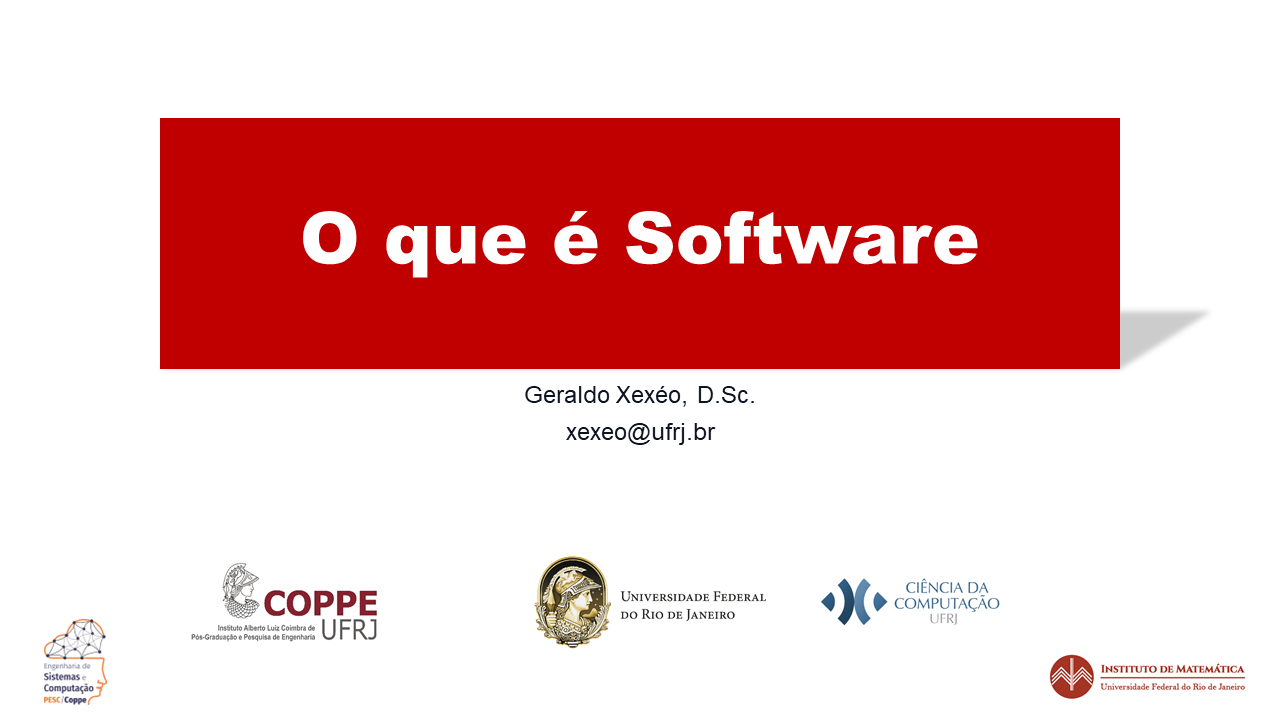
\includegraphics[width=\tam\linewidth,frame]{imagens/capa.png}
    \caption{Um slide de título.}
    \label{fig:titulo}
\end{figure}

Outra boa sugestão é ter um slide, no início, que leve a pensar sobre o conteúdo da aula. Esse slide pode mostrar um problema real onde a técnica poderia ser aplicada, sendo algo do tipo ``como vocês fariam para fazer x?''. Isso seria adequado para uma aula onde se ensina o método PERT/CPM para calcular prazos de um projeto. Já em uma aula de programação inicial, que vai usar exemplos numéricos, poderia ser proposto um problema numérico, como achar números primos.

Ao mostrar um problema é interessante mostrar como ele pode se complicar. Ao mostrar um método de fazer algo que suplantou outro anterior, é interessante mostrar os problemas que o anterior tinha. Deve haver cuidado, porém, na estimativa de tempo, o contexto histórico deve ser limitado a motivação. Se começar do início de tudo, você acabará tendo menos tempo para falar do assunto que deve abordar e poderá perder pontos.

Eu agora também crio mais um slide, que fala sobre a metodologia da aula, e o tamanho da aula em slides e em tempo, como na Figura \ref{fig:metodologia}. Esse slide também mostra como símbolos podem ser usados para passar mensagens. Julgo ser  uma boa ideia mostrar isso também, inclusive porque não é uma prática comum entre os professores e pode surpreender positivamente.

\begin{figure}[htb]
    \centering
    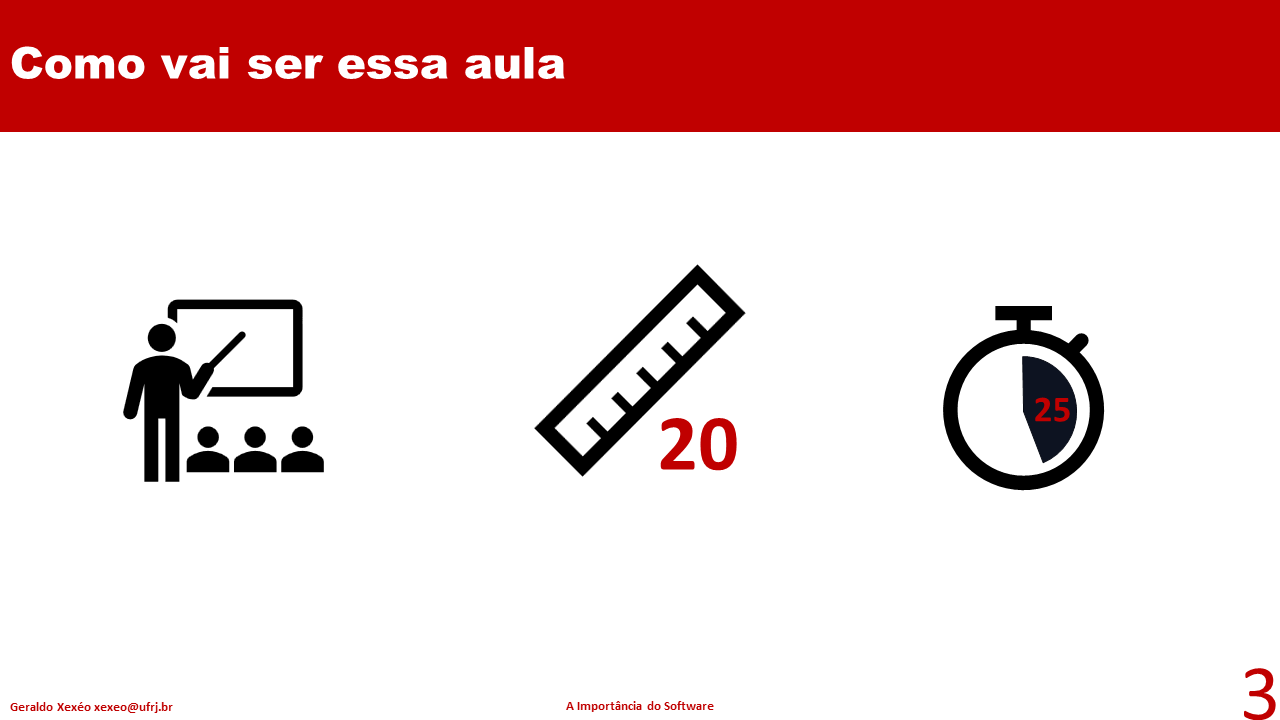
\includegraphics[width=\tam\linewidth,frame]{imagens/metodologia.png}
    \caption{Slide informando o aluno como vai ser a aula.}
    \label{fig:metodologia}
\end{figure}




\subsection{Estilo dos slides de aula}

A melhor estratégia para o estilo dos slides de aula são o fundo branco, letras escuras, e cores para ressaltar. Isso se adequa bem tanto a salas bem iluminadas quanto a salas escuras, para todo tipo de projetor. A Figura \ref{fig:teximag}, apesar de usar o forte grená, me parece bastante adequada. As outras figuras  mostram outros modelos que eu uso e sinto adequados para uma aula. As cores azuis e cinzas, porém, são mais ``fracas'' e podem levar a um pouco de monotonia.

\begin{figure}[hbt]
    \centering
    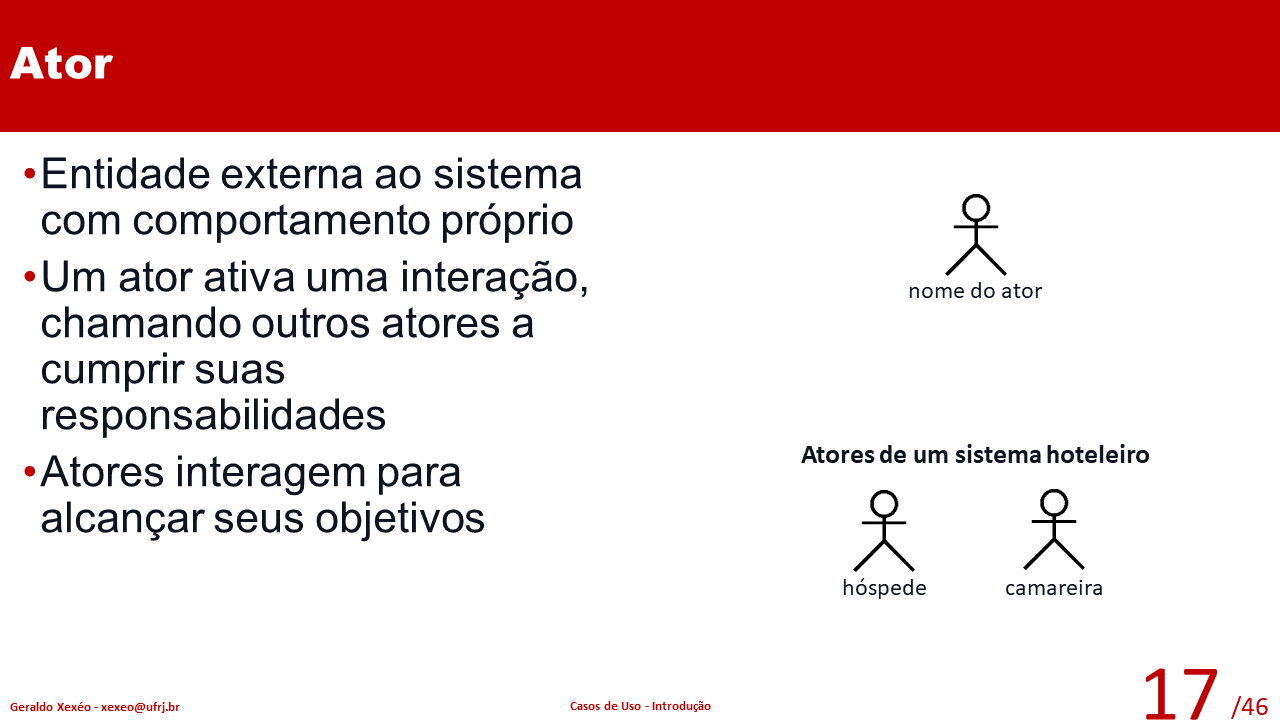
\includegraphics[width=\tam\linewidth,frame]{imagens/slidecomimage.png}
    \caption{Slide com texto e imagem}
    \label{fig:teximag}
\end{figure}

\subsection{Conteúdo dos slides}

Um slide para a aula tem como funções, em ordem decrescente de prioridade:
\begin{enumerate}
    \item servir de referência para o aluno e o professor no momento da aula;
    \item servir de guia para o estudo posterior, e
    \item servir de referência para os tópicos tratados, focando no conteúdo mais importante para a aula.
\end{enumerate}

O conteúdo típico de um slide é um lista de itens que indica o que o professor vai falar naquele momento. Essa lista pode conter exemplos, definições, motivação, dependendo da necessidade do slide.

Outro slide típico contém informações numéricas, na forma de gráficos e tabelas.

Forneça todas as referências, e \textbf{indique a propriedade intelectual de tudo}. Prefira imagens de domínio público ou com licenças amplas, como \textit{Creative Commons}.



\section{Ferramentas}

Esse texto considera 4 ferramentas possíveis para fazer slides acadêmicos:
\begin{itemize}
    \item Power Point
    \item Google Slides
    \item \LaTeX\  com \texttt{beamer}
\end{itemize}

\subsection{Power Point}

Se for usar o \textit{Power Point}, use um estilo e o siga. Evite criar caixas soltas de texto, já que os programa fornece estilos próprios. Coloque os textos nos lugares que são indicados pelas caixas de conteúdo.

É fácil usar fórmulas no \textit{Power Point}, tanto dentro do texto quanto em caixas em separado. Porém, cuidado com a portabilidade, já que as fórmulas não navegam bem entre as versões do Power Point, inclusive do Windows para o MacOS acontecem problemas.

Sempre que for trocar de computador, ``\textbf{inclua as fontes ao salvar}''. Isso exige clicar em ``\textit{more options...}'' em vez de no botão salvar e depois clicar em ``\textit{Tools/Save Options}'', novamente em vez de salvar. Aparecerá a opção ``\textit{Embed fonts in the file}'' e, nela, escolha ``\textit{Embed all characters}''.

Se você usar muitas imagens grandes, o arquivo \texttt{.pptx} pode ficar grande demais. Neste caso você pode escolher qualquer imagem e usar o comando \textit{Picture Format/Compress Pictures}. Nesse comando há uma opção que pode ser ligada ou desligada: ``\textit{Apply only to this picture}''. Use-a para comprimir todas as figuras e salvar bastante espaço. Ela permite escolher vários resoluções.

O Power Point permite criar seções. Elas não tem uma grande utilidade, mas podem ser usadas para organizar melhor a visão do \textit{Slide Sorter}. A Figura \ref{fig:sorter} mostra a visão do \textit{Slide sorter}, que é muito útil para visualizar a apresentação como um todo.

\begin{figure}[tbh]
    \centering
    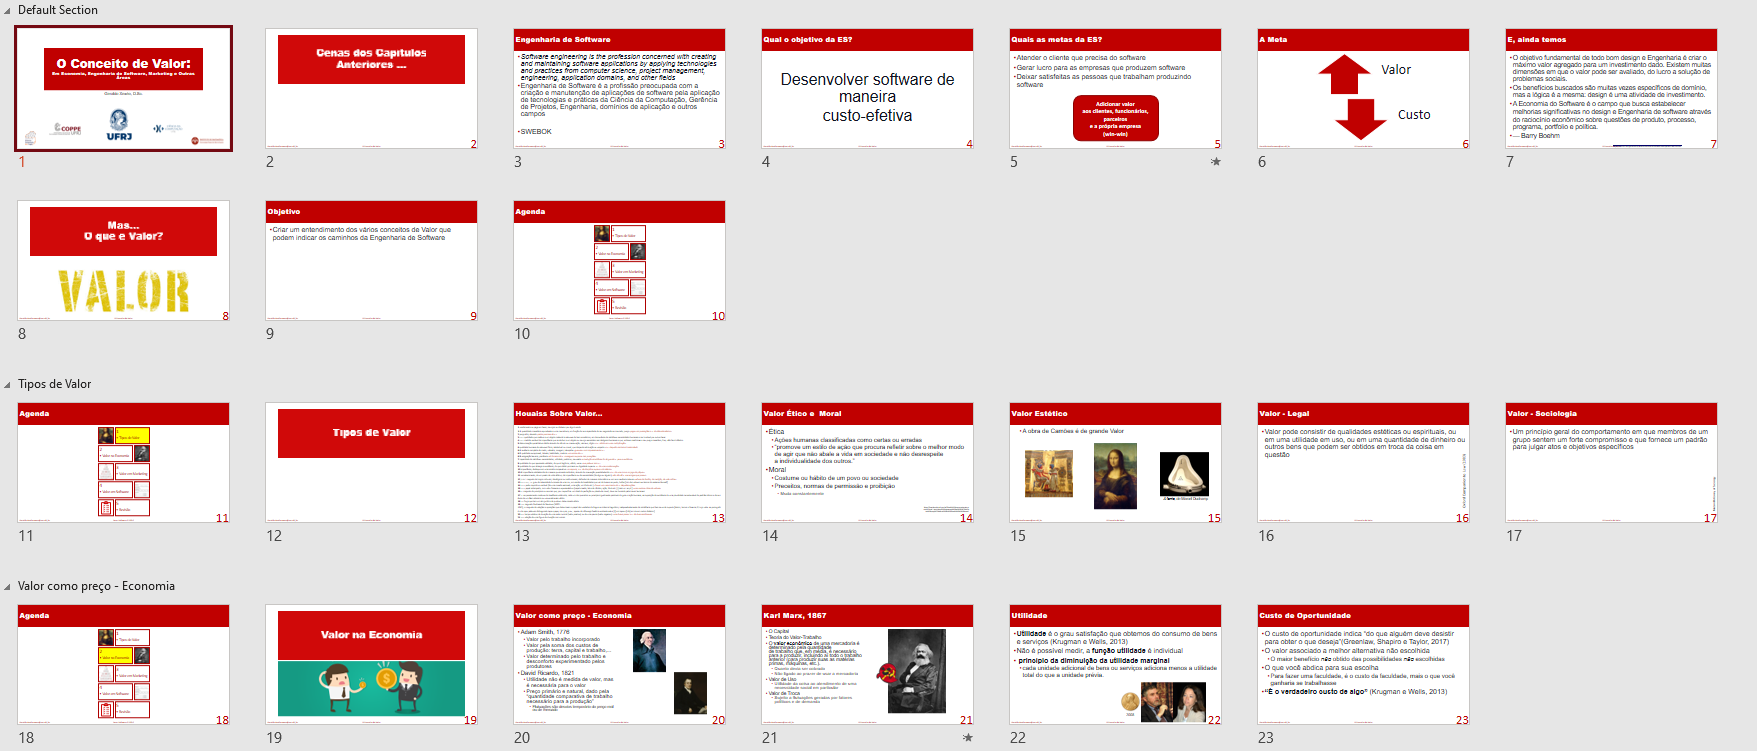
\includegraphics[width=0.7\linewidth]{imagens/slidesorter}
    \caption{Um visão do Slide Sorter do Power Point.}
    \label{fig:sorter}
\end{figure}



\subsection{Google Slides}

Cuidado para não ficar dependente do funcionamento da Internet. Recomendo baixar uma cópia, ou para \textit{Power Point}, ou PDF.








\section{Slides para defesas}

Slides de defesa serão usados em uma ocasião muito formal, e devem seguir as recomendações gerais e ainda as recomendações de estilo para slides de aula, só que com mais cuidado para não causar estranheza à banca.

\subsection{Que slides ter}

A apresentação da tese deve ter como foco a apresentação do trabalho. Para os 50 minutos usados na COPPE, recomendo que pelo menos 50\% do tempo seja usado com o que o aluno fez. A conclusão pode ser rápida, mas não está incluída nesse tempo. O candidato deve tomar cuidado para que o tratamento da revisão e dos trabalhos correlatos não assuma a predominância da apresentação.

Recomenda-se que os seguintes slides sejam usados:
\begin{outline}
    \1 \textbf{Título da dissertação ou tese}, como na Figura \ref{fig:titulo}, contendo ainda o nome do orientado e do orientador;
    \1 \textbf{Agenda} (ou Sumário);
    \1 Um slide de \textbf{título para cada seção};
    \2 Pode ser o slide da agenda colocando ênfase na seção atual, como na Figura \ref{fig:meio};
    \2 Slides de conteúdo, incluindo obrigatoriamente;
        \3 \textbf{Objetivo da tese e sub-objetivos};
        \3 \textbf{Motivação};
        \3 \textbf{Trabalhos correlatos};
        \3 slides \textbf{realmente sobre sua tese ou dissertação};
        \3 \textbf{Contribuições};
        \3 \textbf{Trabalhos futuros};
    \1 \textbf{Referências} bibliográficas;
    \1 Agradecimentos, em especial os obrigatórios, como a CAPES e ao CNPq, e
    \1 Slide de obrigado e abrindo para perguntas
\end{outline}

Na lista acima não tratamos dos slides principais, pois isto depende do estilo da tese. Em teses típicas do PESC são gerados artefatos computacionais que são avaliados de alguma forma. Nesse caso, costuma-se criar duas seções diferenciadas: a proposta e a avaliação. Eu costumo dividir ainda mais, usando três seções típicas, em proposta teórica, implementação, experimento e avaliação. Experimentos muito complicados podem exigir ainda a separação da explicação do experimento e do resultado dos mesmos, havendo então 4 partes.

Note que  eu proponho que o que é chamado normalmente de conclusão tenha duas partes, a contribuição e os trabalhos futuros.

\section{Slides de Apresentações de Artigos}

As apresentações de artigos são o momento onde podemos ser mais criativos com os slides. Isso vem da necessidade de chamar mais atenção em um menor espaço de tempo. É comum que uma apresentação dure apenas 15 minutos.


Uma boa estrutura de slides é:
\begin{itemize}
    \item Título, autores e indicação de como encontrar o artigo;
    \item Apresentação do grupo de pesquisa, já com indicação de contato;
    \item Agenda, que deve ser tratado bem rapidamente e está aqui apenas por uma questão formal;
    \item Apresentação do tema do artigo, do problema, dando motivação e justificativa;
    \item Revisão mínima dos trabalhos correlatos ou antecessores;
    \item Detalhamento da solução que o artigo traz;
    \item Conclusão;
    \item Trabalhos Futuros;
    \item Bibliografia, não será lida, apenas por uma questão formal;
    \item Agradecimentos, em especial os obrigatórios, como a CAPES e ao CNPq, e
    \item Slide de contato que ficará sendo apresentado enquanto se responde as perguntas e que pode indicar outros artigos dos autores relacionados ao tema.
\end{itemize}





\section*{Licença}


Este texto é distribuído com uma licença Creative Commons - Atribuição - NãoComercial - Compartilha Igual 4.0 Internacional.




\begin{center}
   \ccbyncsa
\end{center}

Você tem o direito de:
\begin{itemize}
    \item \textbf{Compartilhar} -- copiar e distribuir o material em qualquer suporte ou formato.
    \item \textbf{Adaptar} -- remixar, transformar, e criar a partir do material.
\end{itemize}

De acordo com os termos seguintes:
\begin{itemize}
    \item \textbf{Atribuição} -- Você deve dar o crédito apropriado, prover um link para a licença e indicar se mudanças foram feitas. Você deve fazê-lo em qualquer circunstância razoável, mas de nenhuma maneira que sugira que o licenciante apoia você ou o seu uso.
    \item \textbf{NãoComercial} --Você não pode usar o material para fins comerciais.
    \item \textbf{CompartilhaIgual} -- Se você remixar, transformar, ou criar a partir do material, tem de distribuir as suas contribuições sob a mesma licença que o original.
    \item \textbf{Sem restrições adicionais} -- Você não pode aplicar termos jurídicos ou medidas de caráter tecnológico que restrinjam legalmente outros de fazerem algo que a licença permita.
\end{itemize}

Mais informações podem ser encontradas em \url{https://creativecommons.org/licenses/by-nc-sa/4.0/deed.pt_BR}


\end{document}